%---------------------------------%
% Article Body
%---------------------------------%
\documentclass[../article.tex, 12pt]{subfiles}
\begin{document}

%---------------------------------%
% Title
%---------------------------------%
\begin{center}
{\bfseries\Huge Cannabis Lab Data | July 2023}
\end{center}

\vspace*{-1\baselineskip}
\begin{center}
{\Large By Keegan Skeate}
\end{center}

%---------------------------------%
% Abstract
%---------------------------------%
\pdfbookmark[1]{Abstract}{Abstract}
\Abstract{\hspace{4ex}Cannabis Intelligence, in its inaugural issue, provides a comprehensive exploration of the cannabis industry using data-driven analysis. This issue delves into the current state of the cannabis industry, identifying key market trends, regulatory shifts, and evolving industry dynamics. It leverages a diverse array of data, encompassing laboratory testing results, market data, regulatory changes, scientific research, and expert opinions. In-depth analysis of laboratory testing data uncovers the nuances of cannabis products, spotlighting the importance of cannabinoids and terpenes in determining product quality and consumer experience. A focus on individual cannabinoids in each issue, supplemented with a detailed review of terpenes, aims to provide a comprehensive understanding of these crucial components of cannabis. This understanding is further enriched by detailed strain profiles that provide a holistic view of various cannabis strains. The value of robust data analysis in the rapidly evolving cannabis industry is demonstrated through sections dedicated to the untapped potential of cannabis data and an in-depth dissection of selected datasets. Emerging trends in the cannabis industry are identified and analyzed, providing a forward-looking perspective to readers. Narratives from industry professionals and answers to reader queries by experts provide invaluable insights into the cannabis industry's trials, triumphs, and intricacies. The inaugural issue concludes with a commitment to upholding the principles of intellectual rigor, academic integrity, and accessibility in the pursuit of cannabis intelligence.
}
% \vspace*{-1\baselineskip}
% \begin{center}
% {\sffamily Dispensary Comparison by Levels of Median Household Income}\vspace*{0.25\baselineskip}\\
% 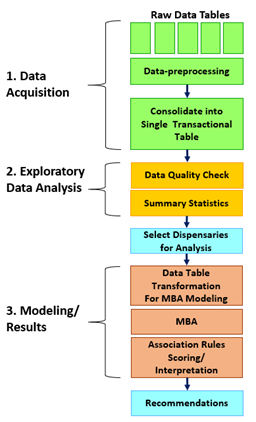
\includegraphics[width=0.8\linewidth]{figures/figure-1.png}
% \end{center}
% \vspace*{0.125\baselineskip}

%---------------------------------%
% Material
%---------------------------------%
\begin{multicols*}{2}

%---------------------------------%
% Introduction
%---------------------------------%
\pdfbookmark[1]{Introduction}{Introduction}
\section{Introduction}
\label{sec:introduction}

\thispagestyle{titlepage}

Welcome to the inaugural issue of Cannabis Intelligence.

In the spirit of intellectual pursuit that characterizes academia's finest, we embark on a journey to unravel the complexities of an industry that continues to burgeon at an unprecedented pace – the cannabis industry. The objective of Cannabis Intelligence is not just to contribute to the scholarly discourse on cannabis but also to create a nexus where data and understanding converge, fostering an environment where decisions – big and small – are dictated by data-driven insights.

As we stand on the precipice of 2023, it is more important than ever to take stock of the cannabis industry's current state. In this issue, we shall illuminate the market dynamics, regulatory changes, and socio-political factors that are shaping the industry today. Through our nuanced narrative, we aim to render a comprehensive image of the cannabis landscape as it stands in the present day and extrapolate the trajectories it might trace in the future.

Data, they say, is the oil of the digital era. As the cannabis industry matures, so does its data. Our goal is to unlock this potential, transforming raw numbers into a wellspring of insights that can propel the cannabis industry to new heights. Our section on cannabis data will illuminate how robust analytics methodologies can uncover latent trends and efficiencies, offering a potent competitive edge to businesses in this space.

Our exploration wouldn't be complete without a deep dive into the science that underpins the industry. Laboratory testing is at the heart of the cannabis industry's quality assurance mechanism, a science that we will demystify for our readers. We will illuminate the myriad parameters tested, the science behind these tests, and their implications for the quality and safety of cannabis products.

One of the most overlooked aspects of the cannabis plant – the terpenes – will find their deserved place in our discussion. Terpenes, though often overshadowed by their cannabinoid counterparts, contribute significantly to the cannabis experience. We aim to provide a comprehensive understanding of these aromatic compounds, elucidating their roles and potential therapeutic benefits.

Every issue of Cannabis Intelligence will shine the spotlight on a different cannabinoid, delving into the biosynthesis, physiological effects, and potential therapeutic uses of these fascinating compounds. In doing so, we hope to offer readers an in-depth understanding of cannabinoids beyond the well-tread path of THC and CBD.

Keeping up with the latest research findings is crucial in any rapidly evolving field. Our Science of Cannabis section will distill the most impactful and recent cannabis research into comprehensive reviews, bringing the most exciting developments in cannabis science to our readers.

In our Strain Profiles section, we aim to illustrate how the unique interplay of genetics, environmental factors, and cultivation techniques endows each strain with distinct characteristics. Through detailed strain analyses, we hope to aid consumers, cultivators, and manufacturers in making informed decisions and fostering a deeper appreciation for this versatile plant.

Our From the Field and Ask the Experts sections aim to foster an active dialogue within the cannabis community. The former will feature candid narratives from industry professionals, providing readers with an authentic glimpse into the trials and triumphs of the cannabis industry. The latter will leverage the collective wisdom of industry experts to address reader queries, stimulating intellectual curiosity and active learning.

Data is most potent when it uncovers hidden trends and patterns. In our Analysis of the Month section, we aim to demonstrate the power of data analytics through a dissection of selected datasets, providing readers with a deeper understanding of the cannabis industry's evolving dynamics.

Finally, by identifying and exploring emerging trends, we aim to equip our readers with a forward-looking perspective. Our Emerging Trends in Cannabis section will enable readers to anticipate changes and seize opportunities in the ever-evolving cannabis landscape.

As we set out on this journey, we pledge to uphold the principles of intellectual rigor, academic integrity, and accessibility. Through Cannabis Intelligence, we aspire to make a meaningful contribution to the understanding of the cannabis industry and foster an informed, engaged, and curious readership.

%---------------------------------%
% Methodology
%---------------------------------%
\pdfbookmark[1]{Methodology}{Methodology}
\section{Methodology}
\label{sec:methodology}

Our exploration of the intricacies of the cannabis industry relies heavily on a rigorous, multidisciplinary methodological approach that draws from economics, data science, and botany, among other fields.

Data Collection

The bedrock of our analyses is the diverse array of data we collate. Our data sources range from lab testing results to market trends and regulatory changes. Data is obtained both from publicly available resources, such as official regulatory databases, and from partnerships with labs and businesses in the cannabis industry.

We employ automated web scraping tools to extract relevant data from online databases and repositories. We also leverage APIs provided by various data sources for efficient, up-to-date data collection. Furthermore, we make use of traditional data collection methods such as surveys and interviews, particularly for our 'From the Field' section.

Data Cleaning and Preprocessing

Given the heterogeneity of our data sources, we place considerable emphasis on data cleaning and preprocessing. We standardize terminologies and units across datasets, deal with missing or inconsistent data, and ensure that our data is fit for analysis.

For instance, when dealing with lab test results, we convert all measures to a standard unit and resolve discrepancies in the naming of cannabinoids and terpenes across different labs.

Analytical Approach

Our analytical approach is underpinned by a blend of descriptive, inferential, and predictive statistical methods. For the 'State of Cannabis' and 'Emerging Trends' sections, we utilize time-series analyses to track changes over time and identify patterns and trends.

In our 'Cannabis Data: An Untapped Resource' section, we deploy machine learning techniques for predictive modelling and clustering analyses. These techniques enable us to uncover hidden patterns and relationships in the data, providing valuable insights for decision-makers in the cannabis industry.

Our 'Analysis of the Month' involves an in-depth dissection of selected datasets using an array of statistical methods tailored to the specific nature and requirements of the data.

Review and Synthesis of Research

Our 'Science of Cannabis', 'Cannabinoid Spotlight', and 'Terpenes 101' sections involve comprehensive literature reviews and syntheses. We collate research findings from a range of sources including peer-reviewed academic journals, preprints, and conference proceedings. We critically evaluate these studies and distill the information into concise, accessible reviews.

Strain Profiling

Our 'Strain Profiles' section is informed by an integration of genetic data, lab test results, and grower information. We present detailed profiles of various strains, offering insights into their unique properties and potential therapeutic benefits.

Expert Engagement

The 'Ask the Experts' section involves soliciting input from experts in the field. We conduct interviews, Q\&A sessions, and panel discussions, focusing on topical issues and reader queries.

Ethical Considerations

Throughout our work, we adhere to ethical guidelines concerning data privacy and research integrity. We ensure that any personally identifiable information is anonymized or excluded from our datasets. In our reviews of research, we ensure to acknowledge all sources and avoid plagiarism.

In sum, the methodological approach underpinning Cannabis Intelligence is both rigorous and adaptable, capable of accommodating the evolving needs of the cannabis industry. We strive to uphold the highest standards of academic integrity in all our work, ensuring that our analyses are both robust and reliable.


%---------------------------------%
% Data
%---------------------------------%
\pdfbookmark[1]{Data}{Data}
\subsection{Data}

The underpinning of our analytical endeavors at Cannabis Intelligence is the diverse array of data we accumulate. This data spans multiple domains and serves as the foundation for our in-depth analyses, profiles, trend identifications, and expert discussions.

Lab Testing Data

The cornerstone of our data is derived from laboratory testing results. These data encompass multiple parameters such as cannabinoid content, terpene profiles, and screenings for contaminants. The raw data is transformed into a standardized form, with units harmonized and terminologies made consistent across different labs and jurisdictions. This vast repository of testing data facilitates our strain profiling, cannabinoid spotlighting, and other related analyses.

Market Data

Understanding the state of the cannabis industry necessitates a firm grasp of market trends. To that end, we collate data from a range of sources including regulatory bodies, industry reports, and market research firms. This market data offers insights into sales trends, product pricing, consumer preferences, and the emergence of new market segments. Such data is integral to our 'State of Cannabis' and 'Emerging Trends in Cannabis' sections.

Regulatory and Legal Data

Given the complex regulatory landscape of the cannabis industry, we maintain an up-to-date collection of regulatory and legal data. This includes state-specific regulations, testing standards, licensing requirements, and legal developments. This data helps contextualize our analyses and guides our discussions on the evolving regulatory environment.

Scientific and Medical Research

Our exploration of the science of cannabis and its medical implications relies on a robust body of academic research. We continually curate peer-reviewed articles, preprints, and conference proceedings from diverse scientific fields including botany, pharmacology, and medicine. This compendium of research forms the basis for our 'Science of Cannabis', 'Cannabinoid Spotlight', and 'Terpenes 101' sections.

Survey and Interview Data

First-hand accounts and expert opinions are invaluable sources of data. We conduct surveys and interviews with industry professionals, researchers, and other stakeholders. The insights gleaned from these interactions add a layer of depth to our analyses and form the backbone of our 'From the Field' and 'Ask the Experts' sections.

Data Management and Analysis

The collected data is managed using state-of-the-art databases that ensure efficient data storage and retrieval. Our data analysis leverages a range of statistical tools and machine learning techniques, tailored to the specific requirements of the data at hand.

Data Ethics

Throughout our data collection and analysis, we adhere to rigorous ethical guidelines. Data privacy is of utmost importance to us, and any personally identifiable information is anonymized or excluded from our datasets. We are committed to transparency and reproducibility in our data analyses, and all data sources are duly acknowledged.

In essence, data serves as the lifeblood of Cannabis Intelligence. It fuels our analyses, enriches our discussions, and anchors us in the realm of evidence-based insights. By meticulously managing and creatively analyzing this data, we strive to illuminate the multifaceted world of the cannabis industry.


%---------------------------------%
% Analysis
%---------------------------------%
\pdfbookmark[1]{Analysis}{Analysis}
\subsection{Analysis}

At Cannabis Intelligence, our analysis serves as the compass guiding our exploration into the cannabis industry. It informs our understanding, shapes our narratives, and uncovers the hidden threads tying the industry's many facets together.

State of Cannabis

Our analysis of the current state of the cannabis industry is an amalgamation of various data sources. By integrating market data, regulatory changes, and industry trends, we paint a comprehensive picture of the industry. We leverage time-series analyses to elucidate evolving patterns, providing our readers with insights into the industry's past trajectories and potential future paths.

Cannabis Data Utilization

Data, when correctly harnessed, provides an unparalleled view into the dynamics of the cannabis industry. Our analysis of this data revolves around identifying key metrics, trends, and relationships that can inform decision-making processes. Through robust statistical analysis and machine learning techniques, we transform raw data into actionable insights.

Lab Testing and Cannabinoid Spotlight

The exploration of laboratory testing data allows us to delve into the nuances of cannabis products. By scrutinizing cannabinoid and terpene profiles, we can shed light on the unique characteristics of various strains and products. Furthermore, our deep dive into specific cannabinoids in each issue gives our readers a comprehensive understanding of these key constituents of cannabis, informed by the latest scientific research.

Terpenes 101

Our analysis of terpene data centers around understanding their role in different cannabis strains. By profiling the terpene content of various strains, we provide readers with an in-depth look at how these compounds contribute to the overall cannabis experience. We also explore the potential therapeutic benefits of terpenes, guided by rigorous scientific research.

Strain Profiles

The profiling of cannabis strains requires an integrative analysis that encompasses genetic data, lab test results, and cultivator information. Our strain profiles provide a holistic view of these strains, offering insights into their unique attributes, potential therapeutic benefits, and consumer experiences.

From the Field and Ask the Experts

Our qualitative analysis of narratives from industry professionals and expert opinions adds depth to our understanding of the cannabis industry. These first-hand accounts provide unique perspectives and insights, complementing our quantitative analyses and enriching our overall narrative.

Analysis of the Month and Emerging Trends

Through our 'Analysis of the Month', we demonstrate the power of data analytics by dissecting selected datasets and highlighting key findings. Additionally, by identifying and analyzing emerging trends, we provide a forward-looking perspective on the future of the cannabis industry.

Data Interpretation and Ethical Considerations

Interpreting our analyses requires a nuanced understanding of the cannabis industry and its intricacies. We ensure our interpretations are grounded in empirical evidence and contextualized within the broader industry landscape.

Throughout our analyses, we adhere to ethical guidelines concerning data privacy and research integrity. Any conclusions we draw are based on robust statistical evidence and transparent methodologies, ensuring the reliability and reproducibility of our findings.

In essence, our analysis at Cannabis Intelligence is a journey of discovery, unearthing insights and patterns that deepen our understanding of the cannabis industry. Through rigorous methodologies, creative data exploration, and careful interpretation, we seek to make this journey an enlightening one for our readers.


%---------------------------------%
% Conclusion
%---------------------------------%
\pdfbookmark[1]{Conclusion}{Conclusion}
\section{Conclusion}
\label{sec:conclusion}

As we reach the end of this inaugural issue of Cannabis Intelligence, we hope to have demonstrated the transformative power of data-driven analysis in understanding the cannabis industry. Through our rigorous methodologies, we've sought to illuminate the multifaceted world of cannabis, from the state of the industry to the science behind its components.

The current state of the cannabis industry is a testament to the remarkable growth and evolution this sector has undergone. By analyzing market trends and regulatory changes, we aim to provide a comprehensive view of the industry's landscape and offer insights into its potential future trajectories.

The value of data in today's digital world cannot be overstated. By harnessing the wealth of data available in the cannabis industry, we can identify key trends, efficiencies, and relationships. It is our belief that robust data analysis can provide a competitive edge to businesses in this rapidly evolving sector.

Lab testing data offers a window into the quality and safety of cannabis products. By demystifying these tests and exploring the cannabinoids and terpenes they quantify, we hope to empower consumers, cultivators, and manufacturers with knowledge that can inform their decisions and deepen their appreciation for this versatile plant.

Our focus on individual cannabinoids and terpenes aims to provide a nuanced understanding of these crucial components of cannabis. By spotlighting a different cannabinoid in each issue and delving into the world of terpenes, we aim to bridge the gap between scientific research and everyday understanding.

Our strain profiles, based on integrated analysis of genetic data, lab test results, and grower information, offer a holistic view of various cannabis strains. We hope that these detailed profiles can facilitate informed choices and foster a deeper appreciation for cannabis's diversity.

The 'From the Field' and 'Ask the Experts' sections bring unique perspectives to our publication, adding depth to our quantitative analyses. These first-hand accounts and expert opinions provide invaluable insights into the trials, triumphs, and intricacies of the cannabis industry.

Lastly, our 'Analysis of the Month' and 'Emerging Trends' sections underscore the value of data analysis in uncovering hidden patterns and anticipating industry changes. It is our aim to equip our readers with a forward-looking perspective, enabling them to seize opportunities in the dynamic cannabis landscape.

As we conclude this issue, we reiterate our commitment to upholding the principles of intellectual rigor, academic integrity, and accessibility in our pursuit of cannabis intelligence. We extend our gratitude to our readers and contributors for embarking on this journey with us, and we look forward to exploring new horizons in the world of cannabis in our forthcoming issues.


%---------------------------------%
% References
%---------------------------------%
\nocite{*}
\pdfbookmark[1]{References}{References}
\bibliography{references}


%---------------------------------%
% End of the Body
%---------------------------------%
\end{multicols*}
\thispagestyle{regular}
\end{document}
